\documentclass[a4paper,10pt]{article}


\usepackage[ngerman]{babel}
\usepackage[T1]{fontenc}
\usepackage[utf8]{inputenc}
\usepackage{setspace}
\usepackage{url}
\usepackage{graphicx}

\usepackage{float}
\usepackage{placeins} % für \FloatBarrier

% Float-Parameter lockern
\renewcommand{\topfraction}{0.95}
\renewcommand{\bottomfraction}{0.95}
\renewcommand{\textfraction}{0.05}
\renewcommand{\floatpagefraction}{0.9}
\setcounter{topnumber}{2}
\setcounter{bottomnumber}{2}
\setcounter{totalnumber}{4}
\onehalfspacing

\title{Aufgabe 1}
\date{\today}


\begin{document}
\maketitle


\section{Einleitung}

Ziel des Logistics Lab ist die effiziente Einsatzplanung eines fahrerlosen Transportsystems zur
Abarbeitung eines gegebenen Auftragspools von Transportaufträgen zwischen mehreren Maschinen.
Als Optimierungskriterium wird die Minimierung der Gesamtbearbeitungszeit betrachtet, welche in der
Produktionsplanung auch Makespan genannt wird.

Die Einsatzplanung stellt ein kombinatorisches Optimierungsproblem dar, dessen exakte Lösung mit
steigendem Problemumfang zunehmend aufwendig wird. Aus diesem Grund wird in dieser Arbeit ein
heuristischer Lösungsansatz verfolgt.

Auf Basis einer Greedy-Heuristik, umgesetzt mit dem Nearest-Neighbor-Algorithmus, sowie darauf aufbauender
zufallsbasierter Varianten werden Einsatzpläne für unterschiedliche Fahrzeuganzahlen berechnet,
miteinander verglichen und kritisch diskutiert.

\section{Problemdefinition und Randbedingungen}

Die betrachtete Problemstellung umfasst die Einsatzplanung einer homogenen Fahrzeugflotte
zur Abarbeitung eines gegebenen, statischen Auftragspools. Die Transportaufträge
bestehen jeweils aus einem Start- und einem Zielort, welche durch Maschinenpositionen innerhalb
eines Hallenlayouts definiert sind.

Die Positionen der Maschinen sind bekannt und fest vorgegeben. Die gesamte Hallenfläche ist frei
befahrbar, wobei die Fahrzeuge stets auf direktem Weg zwischen zwei Maschinen verkehren. Die
zurückgelegte Strecke entspricht somit der euklidischen Distanz zwischen den jeweiligen
Maschinenkoordinaten.

Alle Transportfahrzeuge sind identisch und besitzen eine Transportkapazität von eins, sodass pro
Fahrzeug zu jedem Zeitpunkt maximal ein Transportauftrag bearbeitet werden kann. Jedes Fahrzeug
kann jeden Auftrag ausführen und an einer Maschine sowohl Entladen als auch Beladen. Eine Priorisierung 
oder vorgegebene Reihenfolge der Aufträge liegt
nicht vor. Zu Beginn der Betrachtung befindet sich Fahrzeug $i$ an Maschine $i$.

Zur Reduktion der Problemkomplexität werden weitere idealisierende Annahmen getroffen. Es treten
keine Warte-, Neben- oder Handhabungszeiten auf, Fahrzeugkonflikte werden vernachlässigt und alle
Fahrzeuge bewegen sich mit konstanter Geschwindigkeit. Ziel der Einsatzplanung ist die vollständige
Abarbeitung aller Transportaufträge unter Minimierung des Makespan.


\section{Lösungsansatz zur Einsatzplanung}

Zur Lösung des Einsatzplanungsproblems wird ein heuristischer Ansatz gewählt. Heuristische Verfahren
werden im Kontext von Vehicle-Routing-Problemen häufig eingesetzt, da exakte Optimierungsverfahren
mit einem hohen Rechenaufwand verbunden sind und bei wachsender Problemgröße nur eingeschränkt
praktikabel sind. Ziel ist es daher, mit vertretbarem Rechenaufwand eine qualitativ gute, wenn auch
nicht notwendigerweise optimale Lösung zu ermitteln.

Als Basis dient eine Greedy-Heuristik in Form des Nearest-Neighbor-Algorithmus, welcher in der
Literatur als einfacher und effizienter heuristischer Ansatz zur Lösung von Vehicle-Routing-Problemen
beschrieben wird \cite{harahap2023}. Der Algorithmus trifft lokale Entscheidungen auf
Grundlage minimaler Distanzen und eignet sich insbesondere für praxisnahe Problemstellungen.
Die konkrete Ausgestaltung des k-Nearest-Neighbor-Algorithmus wurde zudem durch methodische Konzepte aus dem Bereich
numerischer Simulation und datengetriebener Modellierung beeinflusst, wie sie unter
anderem in \cite{weiner2021} vermittelt werden.

Aufbauend auf diesem Grundansatz werden zwei Erweiterungen betrachtet, um die Lösungsgüte zu
verbessern und die Abhängigkeit von lokalen Optima zu reduzieren.

\subsection{Greedy Heuristic (GH)}

Bei der klassischen Greedy-Heuristik wählt ein Fahrzeug ausgehend von seiner aktuellen Position
denjenigen offenen Transportauftrag aus. Die Auswahl des nächsten Transportauftrags erfolgt auf 
Basis der euklidischen Distanz zwischen der aktuellen Fahrzeugposition $P(x_j, y_j)$ und der 
Position $P(x_i, y_i)$  eines offenen Transportauftrags, definiert als
$$
  d = \sqrt{(x_i - x_j)^2 + (y_i - y_j)^2}
$$
Nach Abschluss des ausgewählten Auftrags wird die
Fahrzeugposition aktualisiert, und der Auswahlprozess wird fortgesetzt, bis alle Transportaufträge
vollständig abgearbeitet sind. Abbildung~\ref{fig:greedy_heuristic} zeigt exemplarisch die schrittweise Entscheidungslogik der
Greedy-Heuristik anhand der Teilzustände (a) bis (c).

Der Vorteil dieses Ansatzes liegt in seiner einfachen Implementierung, der geringen
Rechenkomplexität sowie der hohen Nachvollziehbarkeit der resultierenden Einsatzpläne.
Aufgrund der lokalen Entscheidungsstrategie kann bei Greedy-Verfahren das Erreichen eines global
optimalen Einsatzplans nicht sichergestellt werden.

\begin{figure}[htbp]
  \centering
  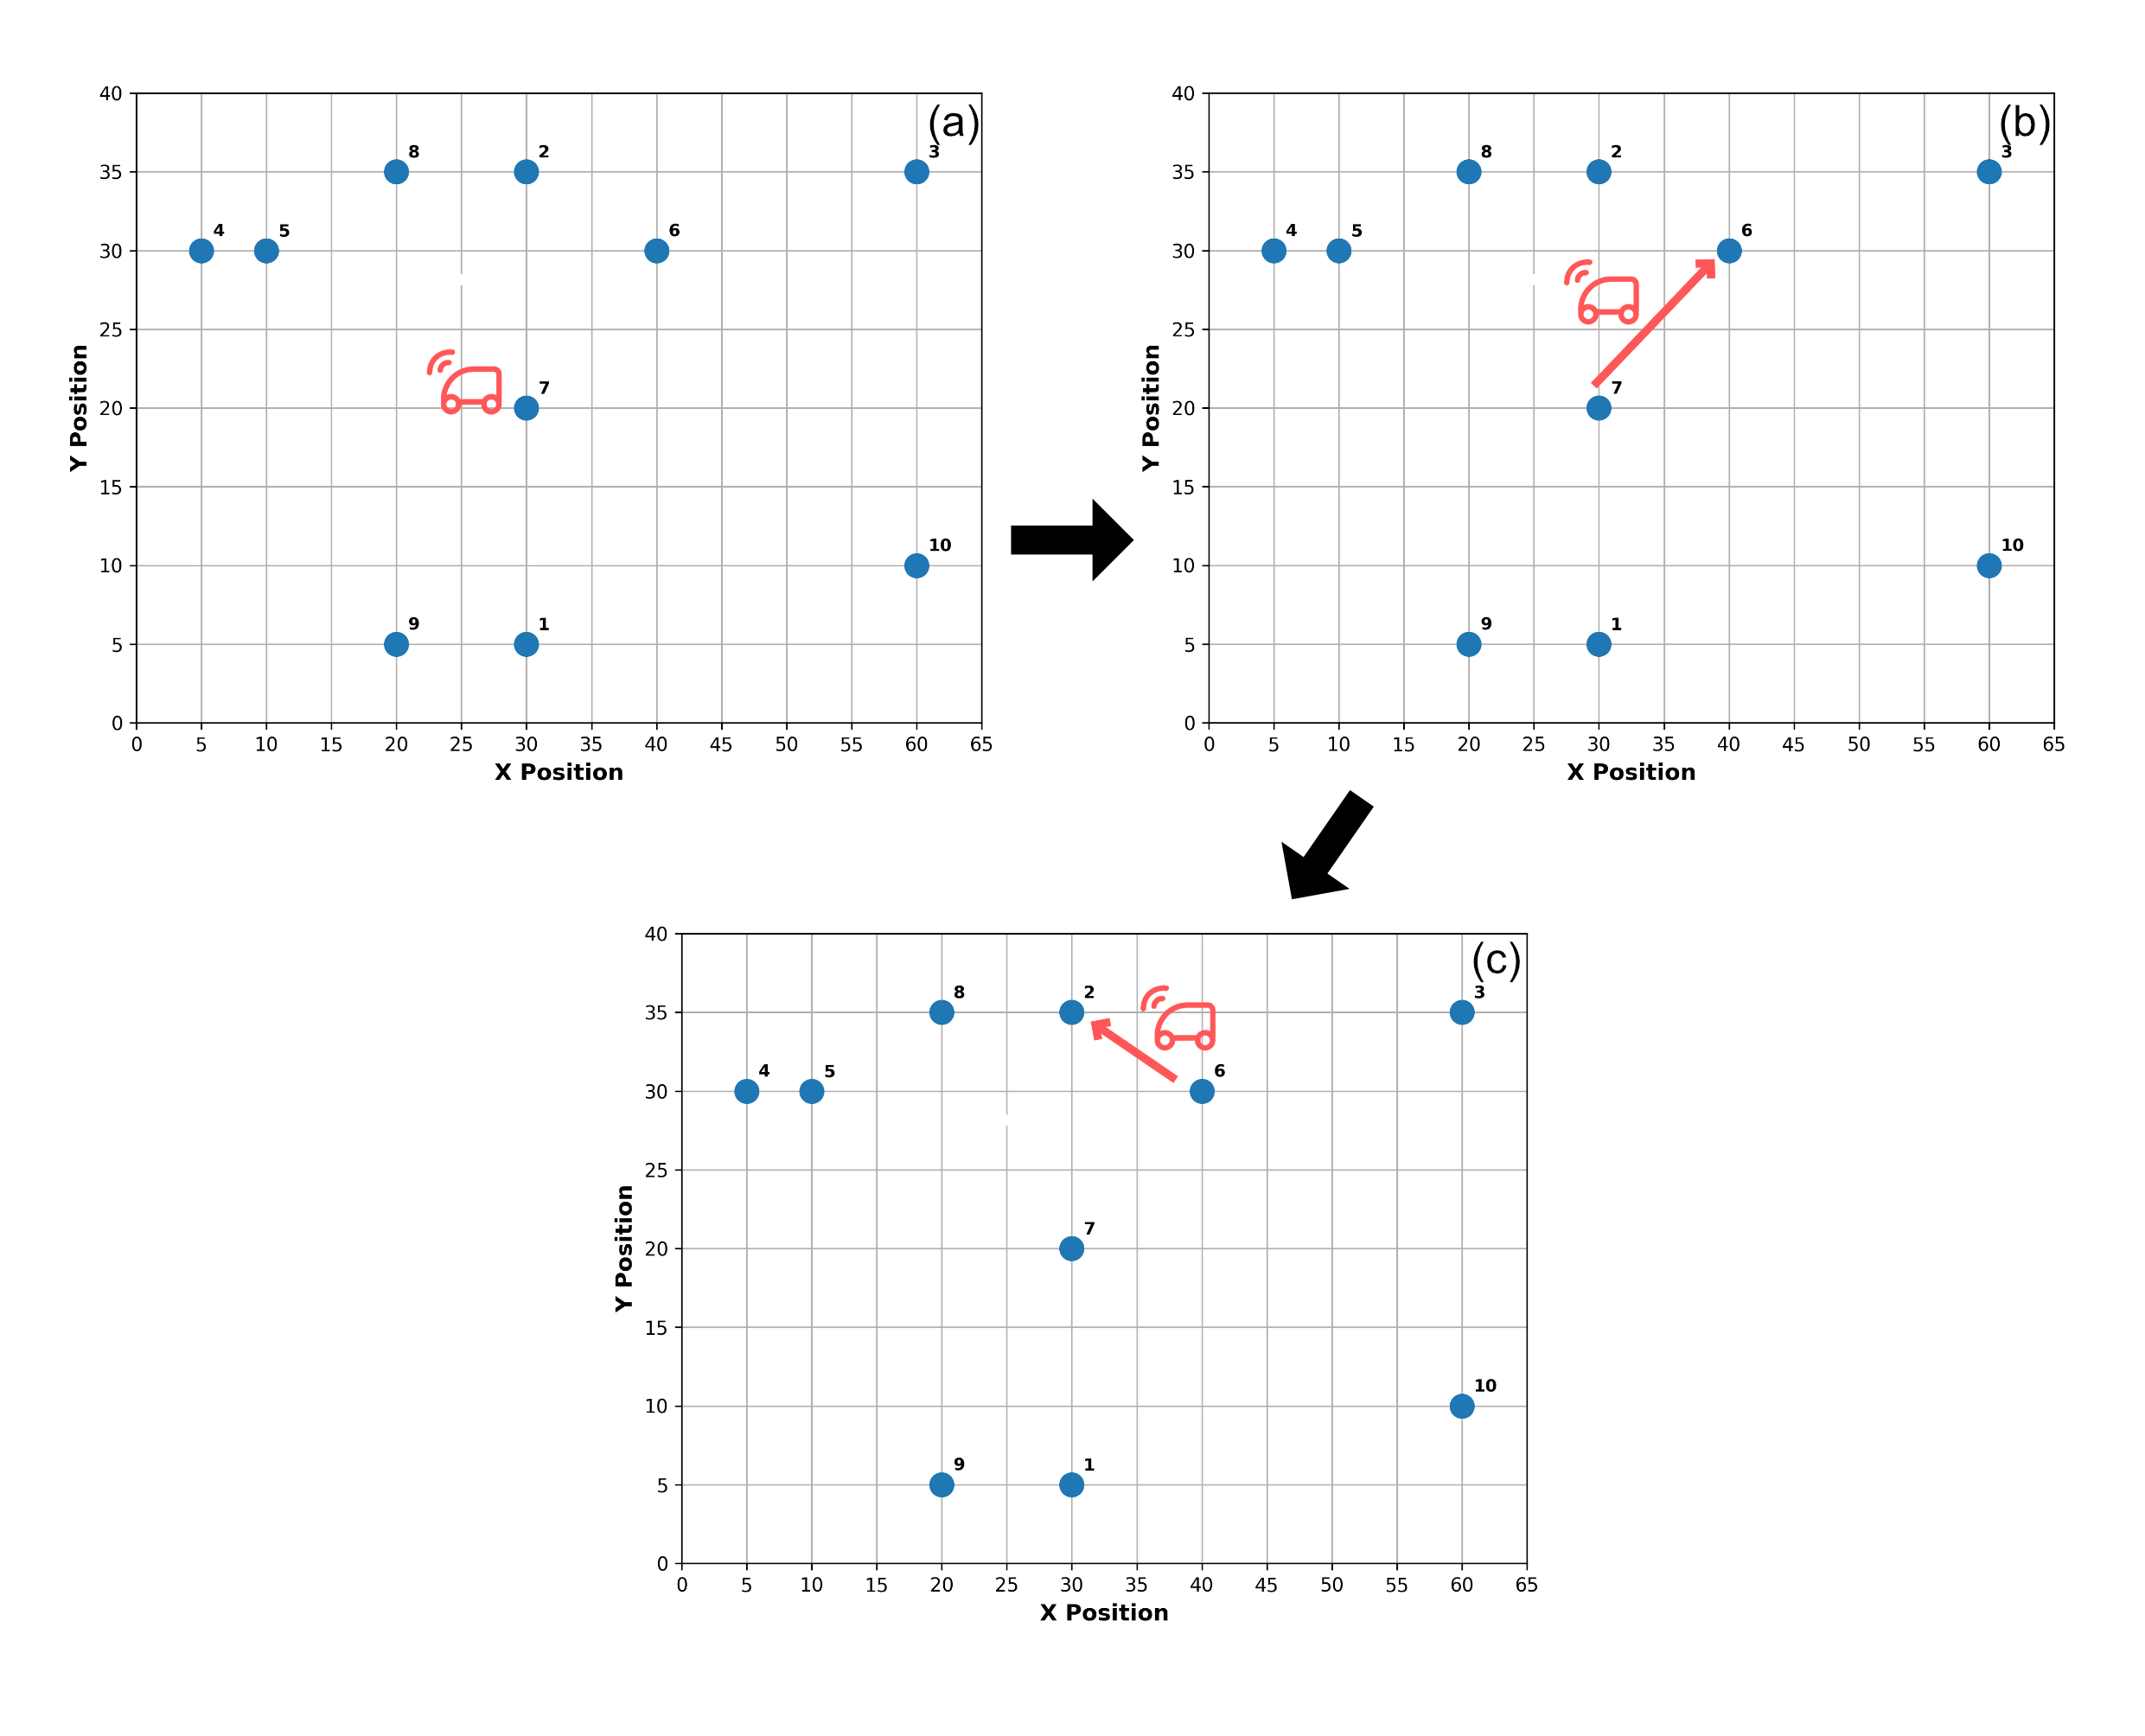
\includegraphics[width=0.85\textwidth]{figures/gh.png}
  \caption{Schematische Darstellung der Entscheidungsabfolge der Greedy-Heuristik.
  Ausgehend von der initialen Fahrzeugposition (a) wird iterativ der jeweils nächstgelegene
  Transportauftrag auf Basis der euklidischen Distanz ausgewählt (b, c).}
  \label{fig:greedy_heuristic}
\end{figure}
\FloatBarrier



\subsection{Randomized Greedy Heuristic (RGH)}

Um die Einschränkung der klassischen Greedy-Heuristik auf lokale Entscheidungsregeln zu reduzieren,
wird der Ansatz um eine Zufallskomponente erweitert. Anstatt stets denjenigen Transportauftrag mit
minimaler euklidischer Distanz auszuwählen, wird aus einer Menge der $k$ nächstgelegenen offenen
Transportaufträge zufällig ein Auftrag bestimmt. Die Bestimmung dieser Kandidatenmenge erfolgt
analog zum \emph{$k$-Nearest-Neighbor}-Algorithmus auf Basis der euklidischen Distanz.

Durch diese Zufälligkeit wird der Lösungsraum stärker erkundet, sodass alternative Einsatzpläne entstehen können, die mit der klassischen
Greedy-Heuristik nicht erreichbar sind. Der Parameter $k$ beeinflusst dabei maßgeblich das
Verhältnis zwischen lokaler Optimierung und Diversität der erzeugten Lösungen.

Zur Gewährleistung reproduzierbarer Ergebnisse wird ein fester Zufalls-Seed verwendet. Die
Randomized Greedy Heuristic stellt somit einen Kompromiss zwischen der einfachen Struktur der
Greedy-Heuristik und einer verbesserten Berücksichtigung globaler Lösungsalternativen dar.

Abbildung~\ref{fig:rgh_sequence} veranschaulicht die Entscheidungslogik der Randomized Greedy
Heuristic anhand der Teilzustände (a) bis (c). Dabei wird der nächste Transportauftrag nicht
deterministisch gewählt, sondern zufällig aus einer Kandidatenmenge der $k$ nächstgelegenen
Transportaufträge ausgewählt.

\begin{figure}[htbp]
  \centering
  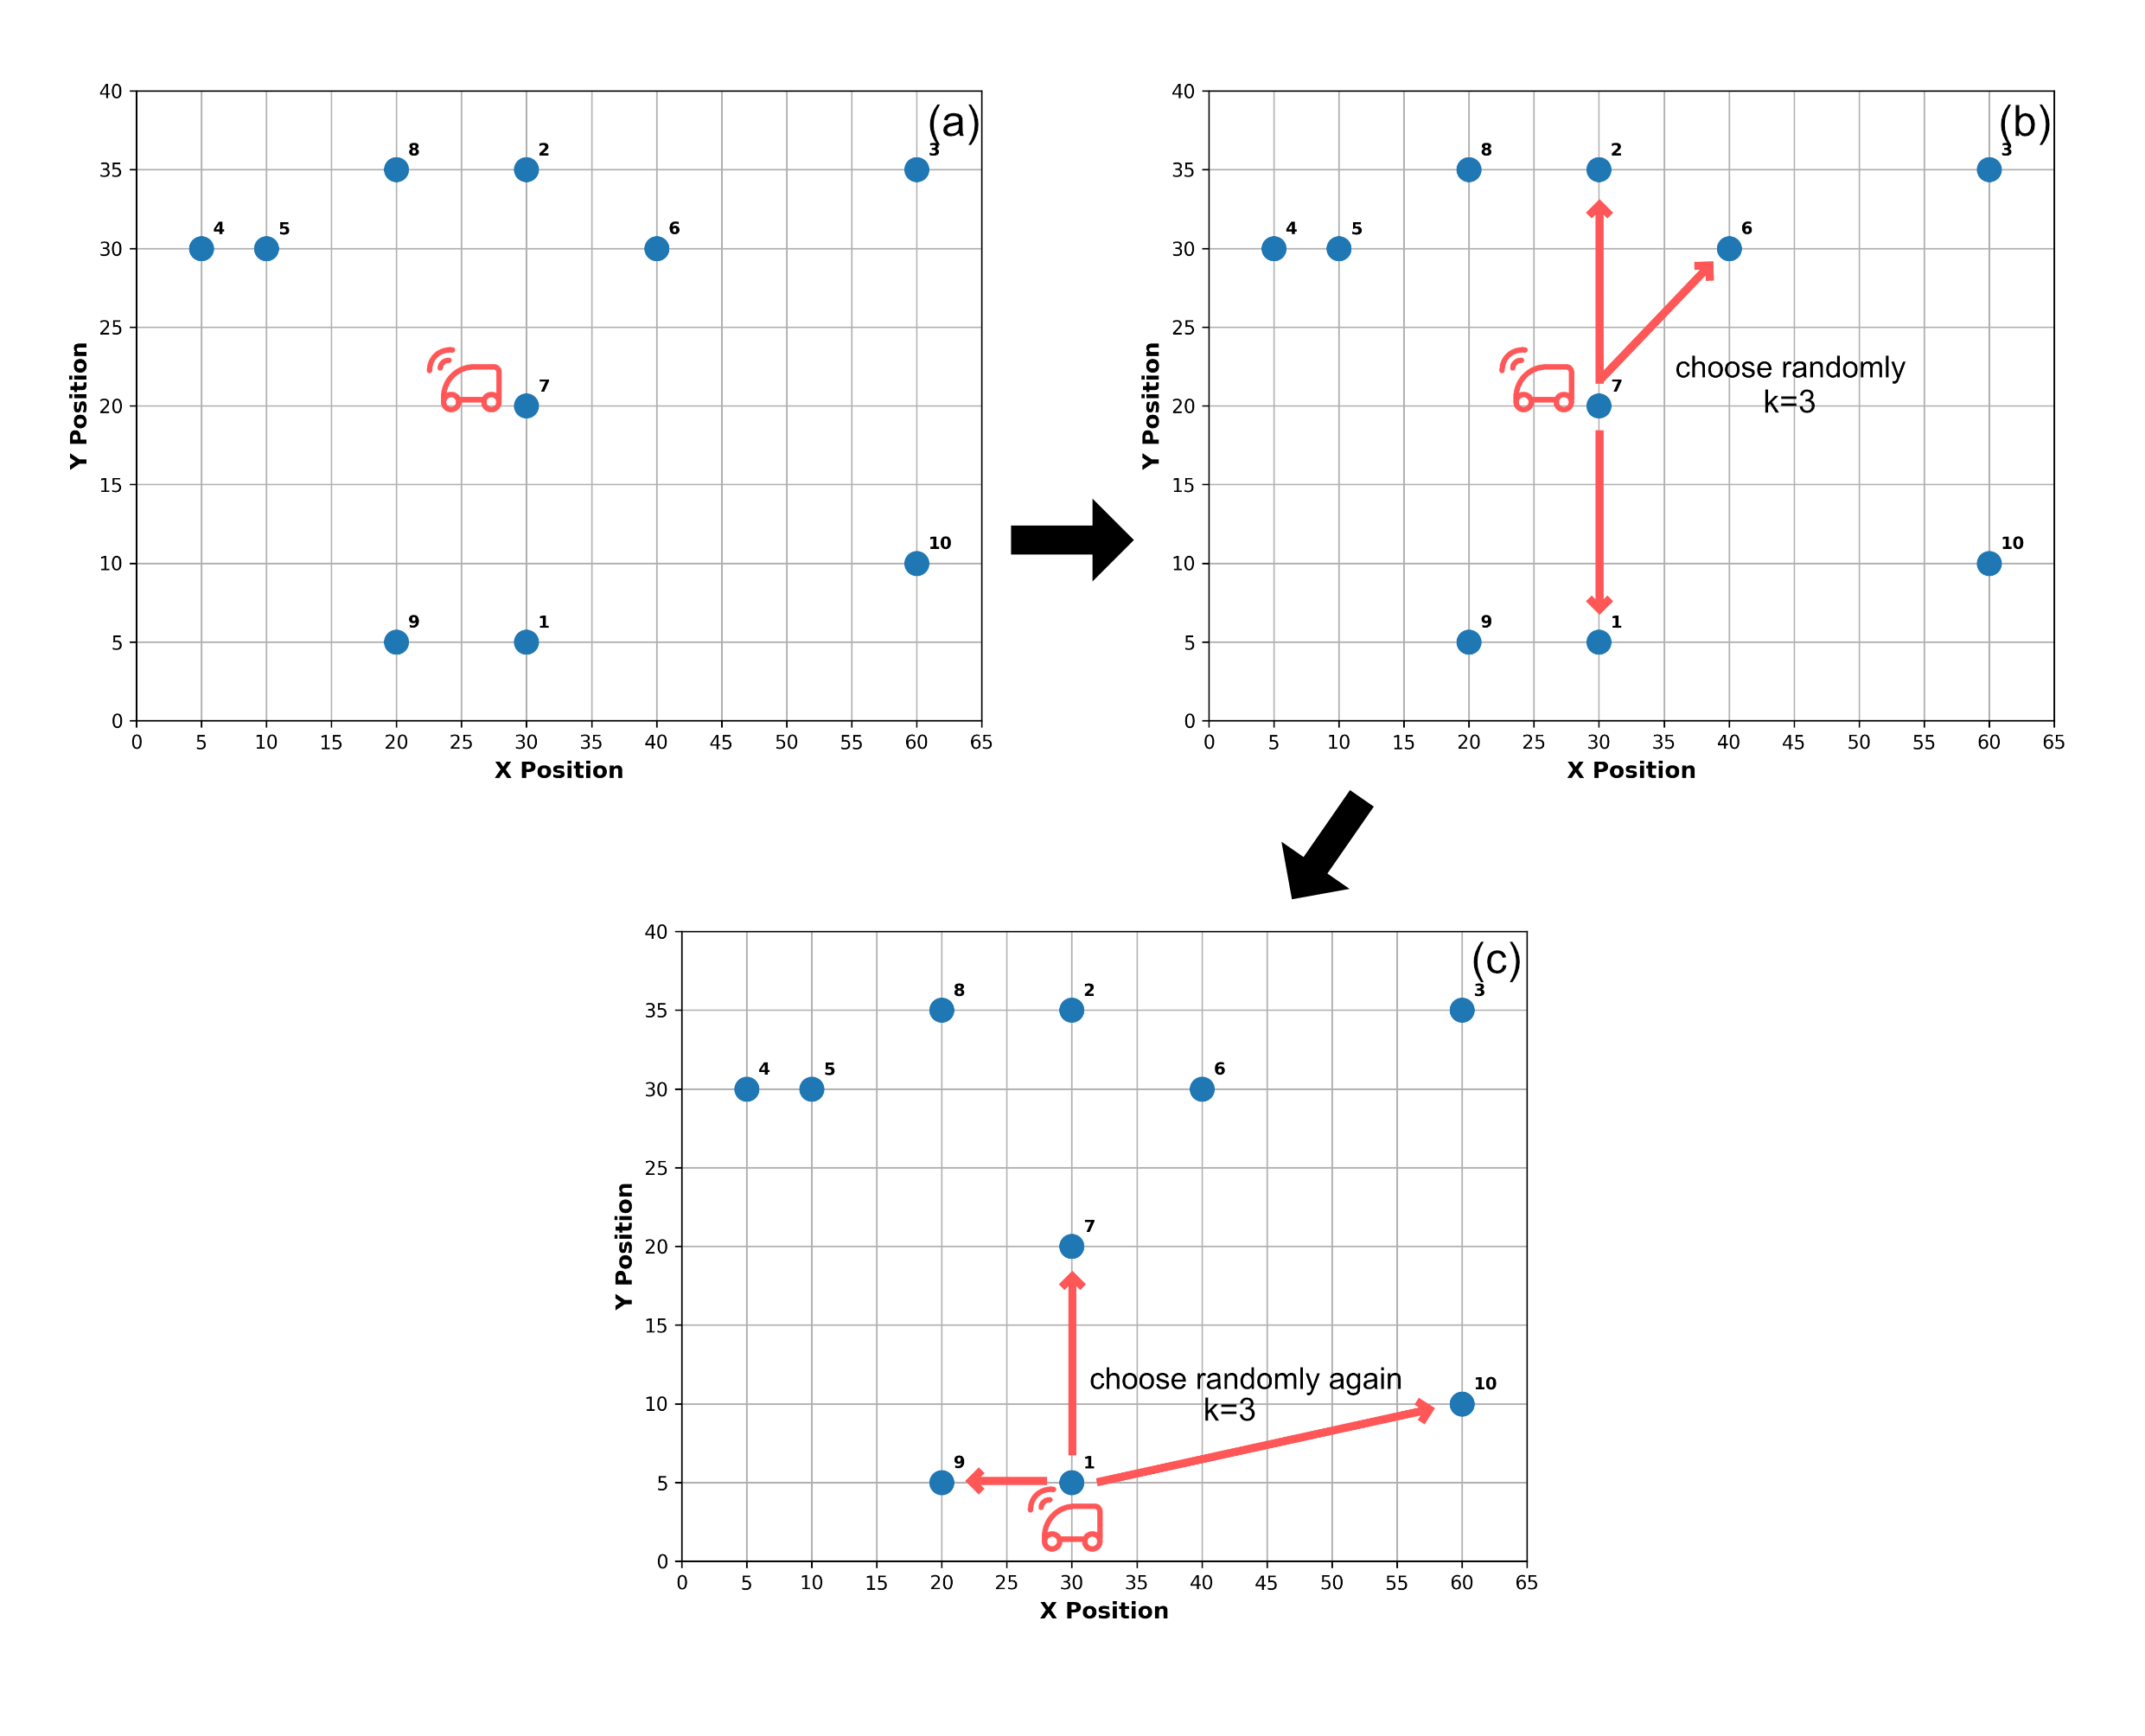
\includegraphics[width=0.85\textwidth]{figures/rgh.png}
  \caption{Schematische Darstellung der Entscheidungsabfolge der Randomized Greedy Heuristic.
  Ausgehend von der initialen Fahrzeugposition (a) wird in jedem Schritt zufällig aus den $k$
  nächstgelegenen offenen Transportaufträgen ausgewählt (b, c); hier exemplarisch mit $k=3$.}
  \label{fig:rgh_sequence}
\end{figure}


\subsection{Multistart Randomized Greedy Heuristic (MRGH)}

Die Multistart Randomized Greedy Heuristic erweitert den zuvor beschriebenen Ansatz, indem die
Randomized Greedy Heuristic mehrfach mit unterschiedlichen Zufalls-Seeds ausgeführt wird. Jede
Ausführung startet dabei mit identischen Anfangsbedingungen, unterscheidet sich jedoch in der
zufallsbasierten Auswahl der Transportaufträge.

Durch die wiederholte Anwendung des Algorithmus entsteht eine Menge unterschiedlicher
Einsatzpläne, welche den Lösungsraum weiter abdecken als eine einzelne Ausführung.
Der Multistart-Ansatz erhöht somit die Wahrscheinlichkeit, Lösungen zu finden, die näher am
globalen Optimum liegen, ohne die grundlegende Struktur des heuristischen Verfahrens zu verändern.
Gleichzeitig bleibt der Rechenaufwand im Vergleich zu exakten Optimierungsverfahren moderat, da
die einzelnen Algorithmusdurchläufe unabhängig voneinander ausgeführt werden können.

Abbildung~\ref{fig:mrgh_sequence} verdeutlicht das Prinzip des Multistart-Ansatzes: Die Randomized
Greedy Heuristic wird mehrfach mit identischen Anfangsbedingungen, jedoch unterschiedlichen
Zufalls-Seeds ausgeführt. Dadurch entstehen verschiedene Einsatzpläne, aus denen anschließend die
beste Lösung gemäß Validierungsscore ausgewählt wird.

\begin{figure}[htbp]
  \centering
  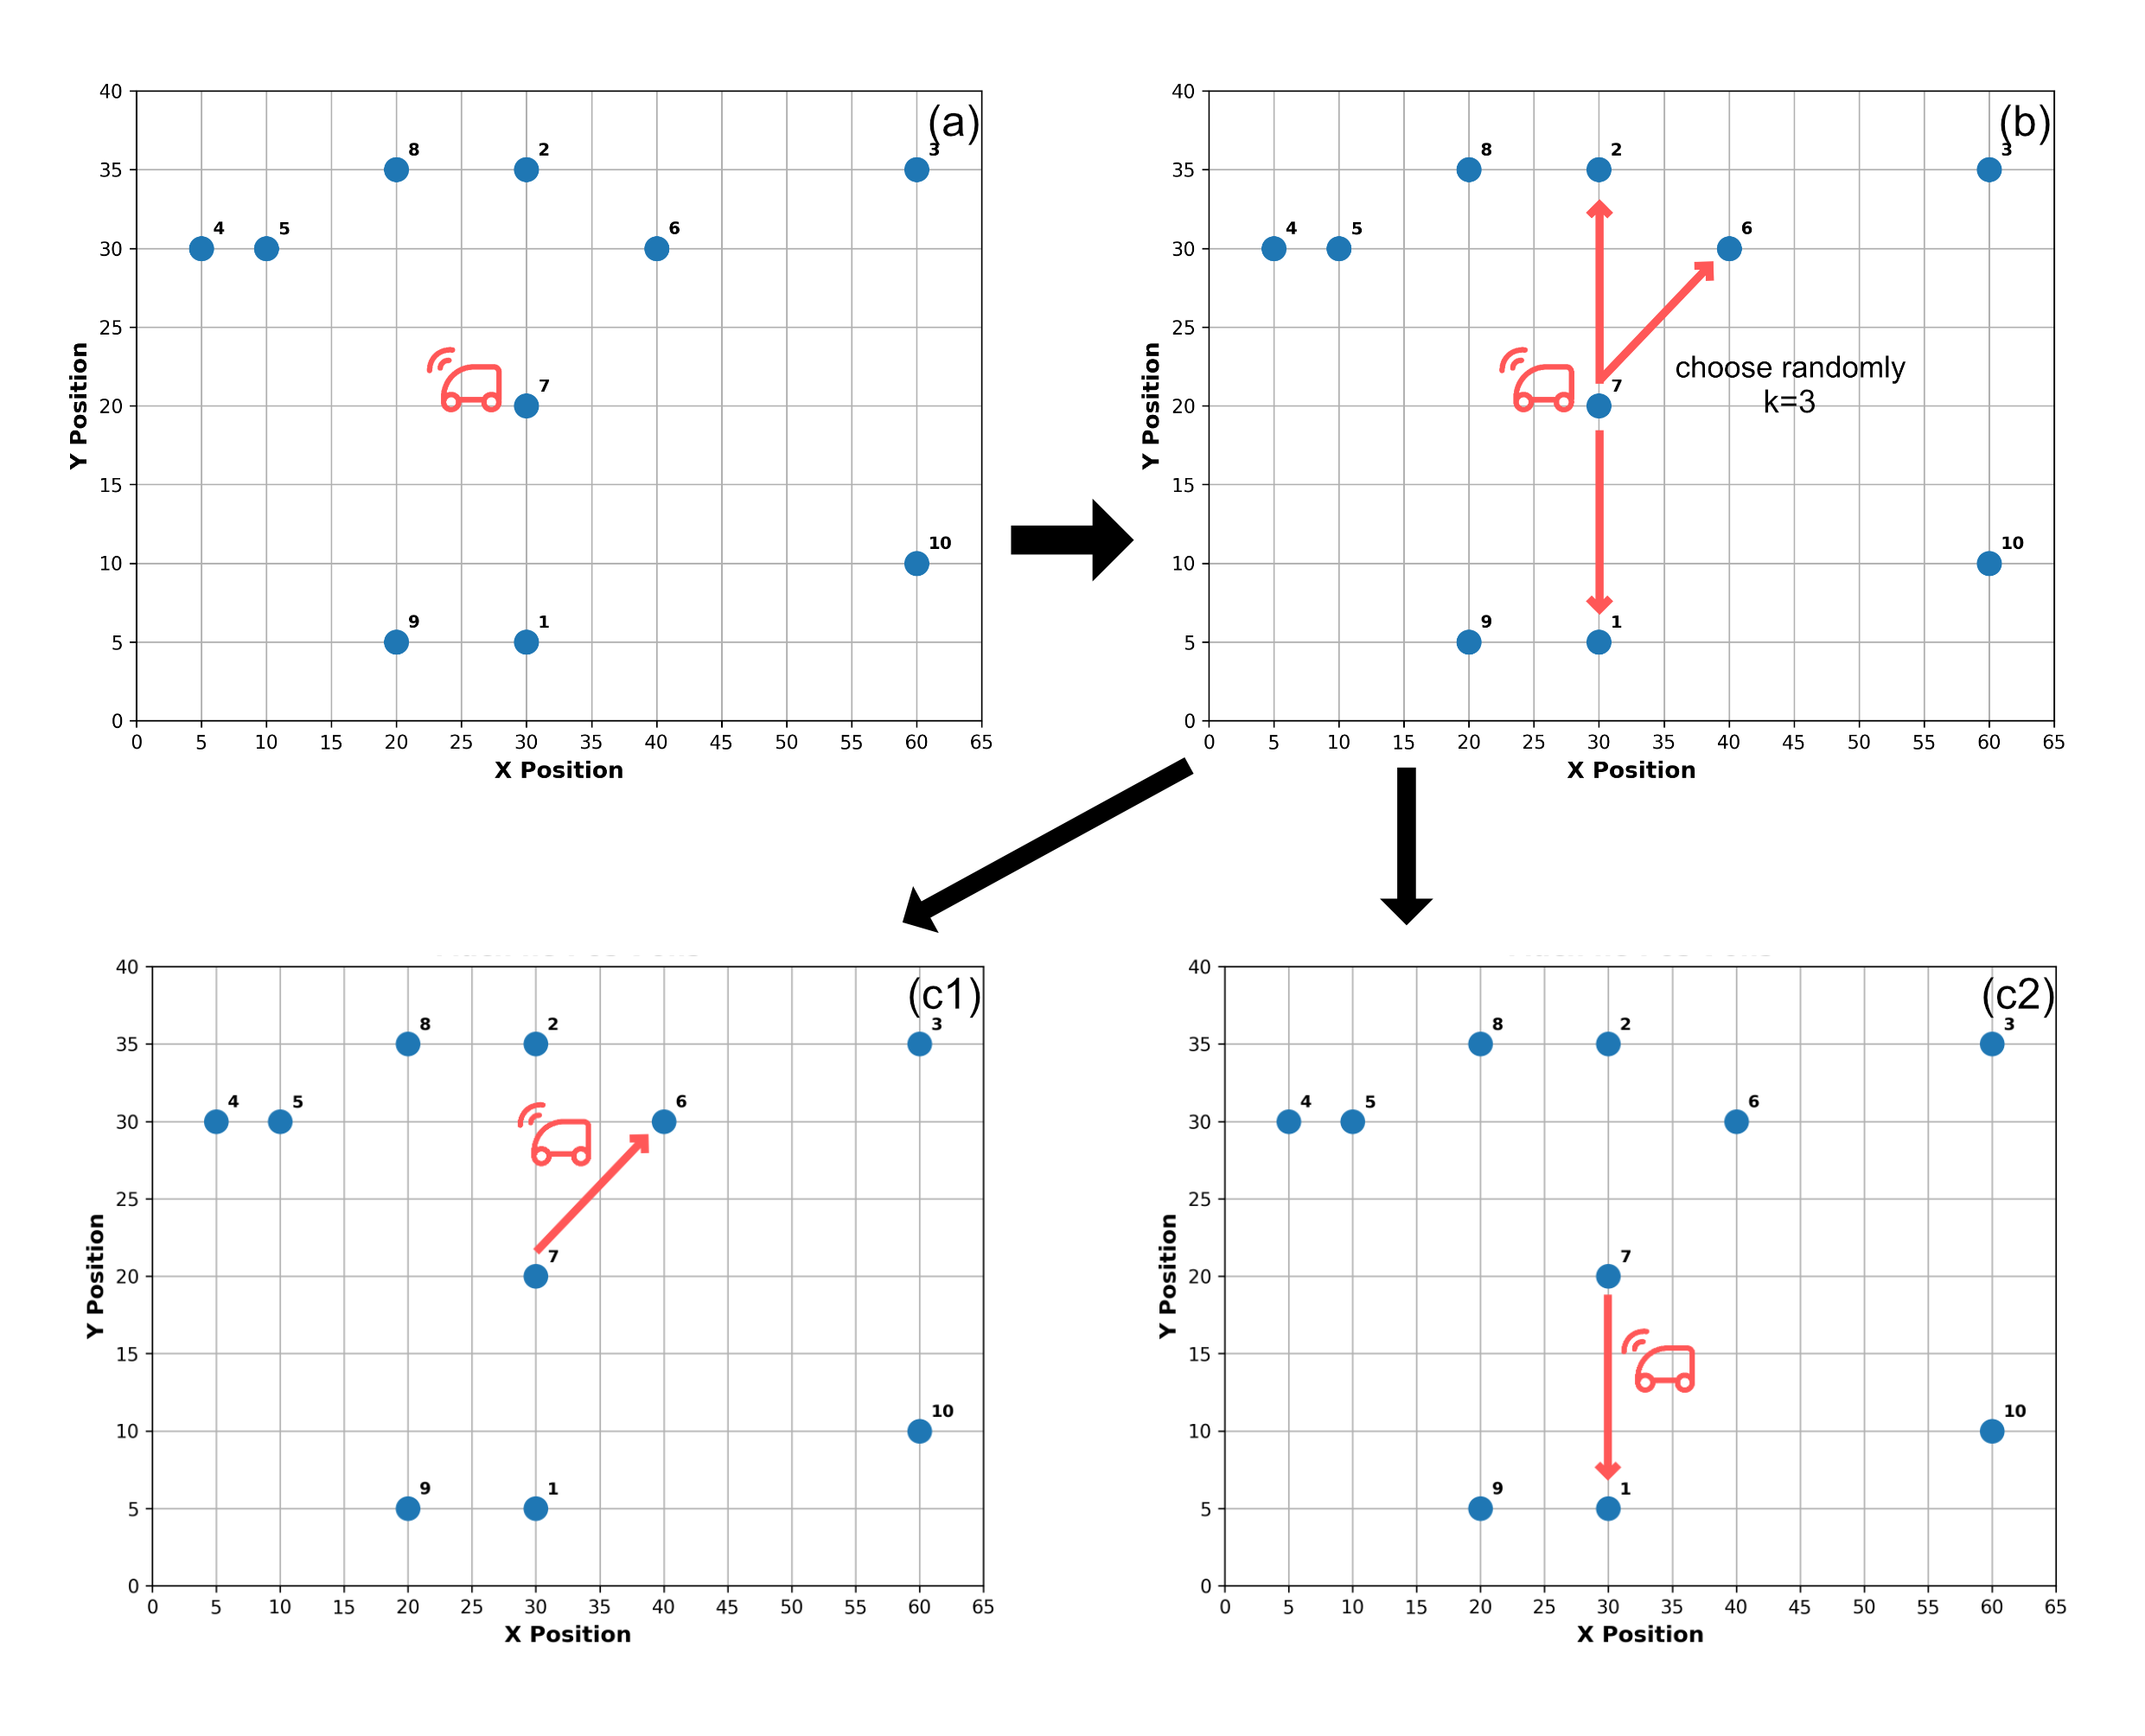
\includegraphics[width=0.90\textwidth]{figures/mrgh.png}
  \caption{Schematische Darstellung des Multistart-Prinzips der MRGH. Die RGH wird mehrfach mit
  unterschiedlichen Zufalls-Seeds ausgeführt (hier exemplarisch zwei Seeds bei $k=3$), wodurch
  verschiedene Einsatzpläne entstehen. Die finale Lösung ergibt sich aus der Auswahl der besten
  Realisierung anhand des Validierungsscores.}
  \label{fig:mrgh_sequence}
\end{figure}

\subsection{Einordnung des heuristischen Ansatzes}

Neben heuristischen Greedy-Verfahren existieren weitere Lösungsansätze die auf einer globalen Modellierung 
des Problems basieren. Dazu zählen insbesondere graphbasierte Optimierungsverfahren sowie Metaheuristiken.

Ein bekanntes graphbasiertes Verfahren stellt das Chinese-Postman-Problem dar, bei dem durch eine
globale Betrachtung des zugrunde liegenden Graphen eine optimale Rundtour bestimmt wird.
Darüber hinaus werden in der Literatur Metaheuristiken wie der Ameisenalgorithmus
(Ant Colony Optimization) zur Lösung von Routing-Problemen eingesetzt.

Derartige Verfahren können global bessere Lösungen liefern, sind jedoch mit einem deutlich höheren
Modellierungs- und Rechenaufwand verbunden und daher für praxisnahe Anwendungen häufig nur
eingeschränkt praktikabel.


\section{Implementierung}

Die Implementierung der beschriebenen Heuristiken erfolgte in der Programmiersprache Python und
ist in einem öffentlich zugänglichen GitHub-Repository\footnote{\url{https://github.com/anh-lxn/logisticsLab}} dokumentiert.
Zur Gewährleistung einer übersichtlichen und modularen Struktur wurde ein objektorientierter Ansatz gewählt.

Die grundlegenden Komponenten der Einsatzplanung sind in separaten Klassen gekapselt. Die Klasse
\texttt{Car} repräsentiert ein einzelnes Transportfahrzeug und verwaltet dessen aktuelle Position sowie
den aktuellen Transportzustand. Das zugrunde liegende Transportnetzwerk, bestehend aus
Maschinenpositionen und Transportaufträgen, wird durch die Klasse \texttt{Network} modelliert.
Hierbei werden unter anderem die euklidischen Distanzen zwischen den Maschinenpositionen in einer
Distanzmatrix vorab berechnet.

Die eigentliche Einsatzplanung und Ausführung der heuristischen Algorithmen erfolgt innerhalb der
Klasse \texttt{Simulation}, welche die verschiedenen Heuristiken auf das Netzwerk anwendet und
gültige Einsatzpläne erzeugt. Wiederkehrende Hilfsfunktionen, beispielsweise zur Datenverarbeitung
oder Ergebnisaufbereitung, sind in einer separaten \texttt{utils.py}-Datei zusammengefasst.

Das Zusammenführen der einzelnen Komponenten sowie die Durchführung der Simulationen für die
unterschiedlichen Szenarien erfolgt in einem zentralen Jupyter Notebook \texttt{main.ipynb}. Dieses
dient gleichzeitig der Auswertung und Visualisierung der Ergebnisse.

Zur Überprüfung der formalen Korrektheit und zur Bewertung der erzeugten Einsatzpläne wurde das
vom Lehrstuhl bereitgestellte Validierungsskript \texttt{validations.py} verwendet und für die eigene Implementierung
entsprechend angepasst.


\section{Ergebnisse und Auswertung}

\subsection{Validierungsergebnisse}

Die Validierungsergebnisse für die Szenarien mit 1, 5 und 10 Fahrzeugen sind in
Abbildung~\ref{fig:validation_results} dargestellt. Gezeigt sind jeweils die erzielten
Validierungsscores der untersuchten Heuristiken, der vom Kurs vorgegebene Referenzwert
sowie die zugehörige Anzahl an Leerfahrten.

\begin{figure}[htbp]
  \centering
  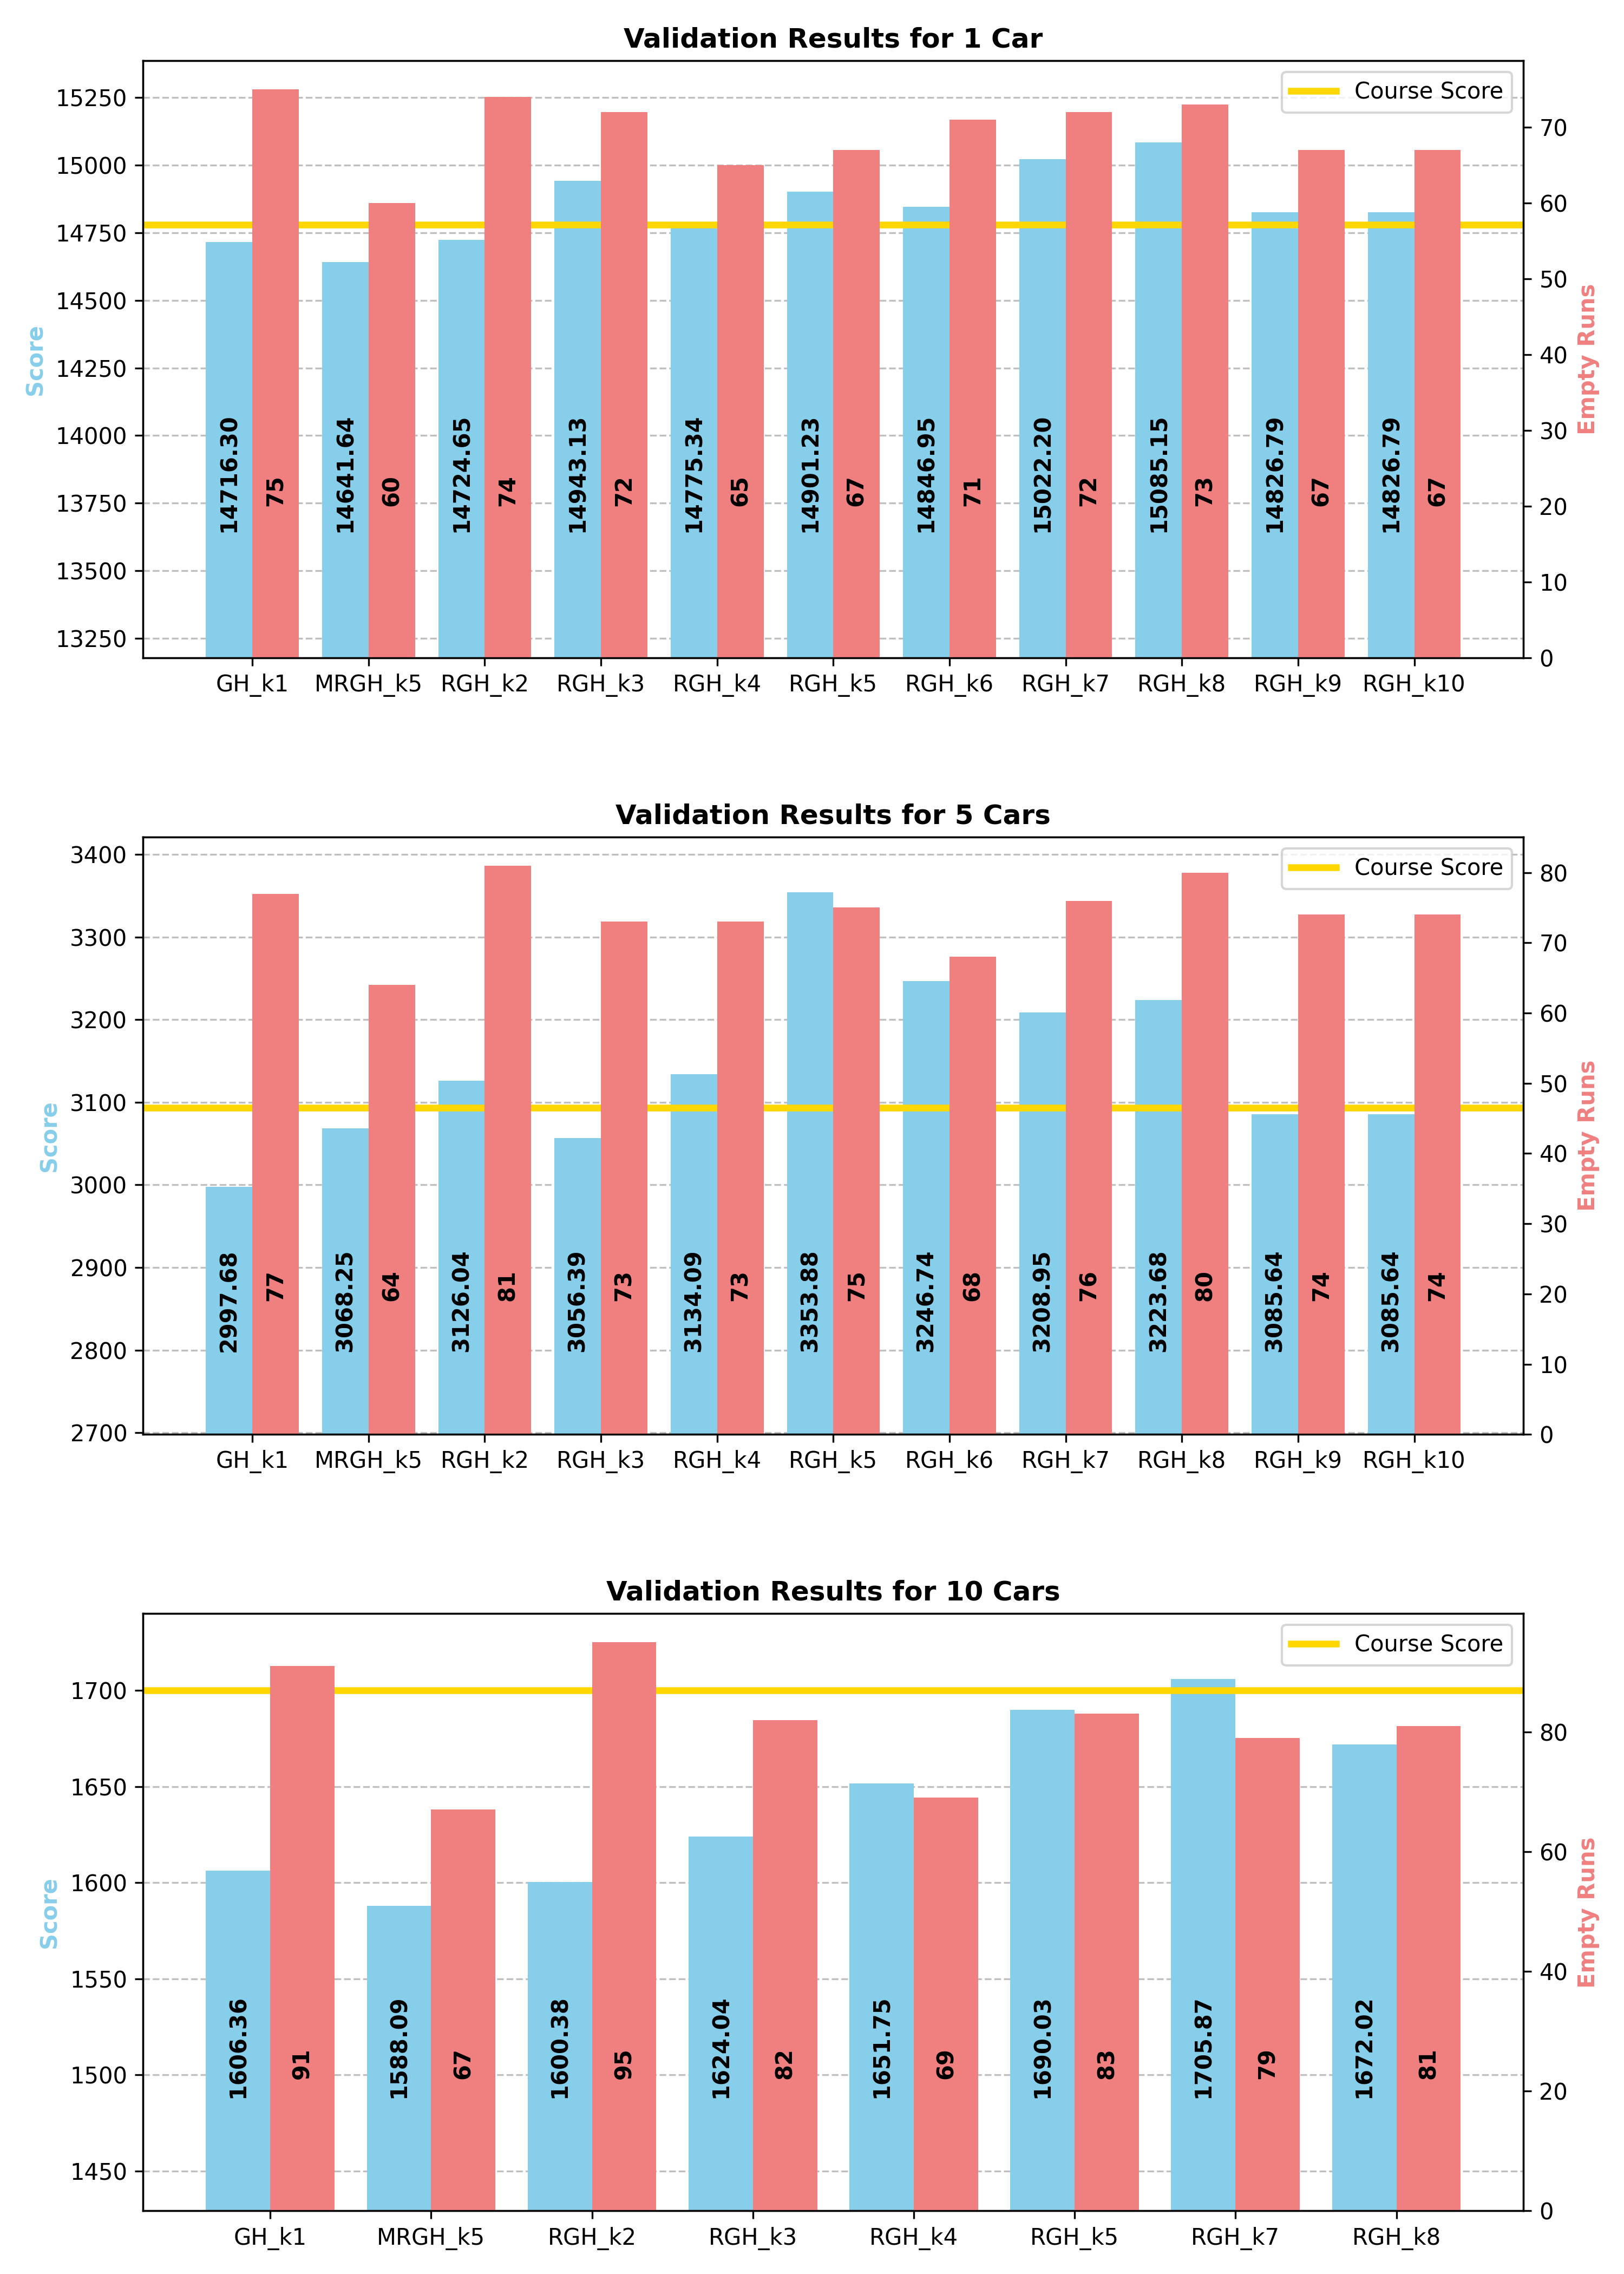
\includegraphics[width=\textwidth]{figures/validation_results.png}
  \caption{Validierungsergebnisse für die Szenarien mit 1, 5 und 10 Fahrzeugen. Dargestellt
  sind die Validierungsscores der untersuchten Heuristiken sowie die jeweilige Anzahl an
  Leerfahrten. Der Kurs-Referenzwert ist als horizontale Linie eingezeichnet.}
  \label{fig:validation_results}
\end{figure}

\subsubsection{Szenario mit einem Fahrzeug}

Im Szenario mit einem Fahrzeug erzielt die Multistart Randomized Greedy Heuristic (MRGH) mit
$k=5$ den besten Validierungsscore. Der erreichte Wert liegt unter dem Kurs-Referenzwert, was
auf eine effizientere Abarbeitung der Transportaufträge hinweist. Gleichzeitig weist diese
Konfiguration eine vergleichsweise geringe Anzahl an Leerfahrten auf.

Die Ergebnisse der klassischen Greedy-Heuristik sowie der Randomized Greedy Heuristic mit
kleineren $k$-Werten fallen in diesem Szenario schlechter aus. Bei nur einem Fahrzeug haben
frühe lokale Entscheidungen einen besonders starken Einfluss auf den weiteren Routenverlauf.

\subsubsection{Szenario mit fünf Fahrzeugen}

Für das Szenario mit fünf Fahrzeugen liefert die klassische Greedy-Heuristik (GH) den besten
Validierungsscore. Im Vergleich zu den anderen Varianten zeigt sich, dass die einfache
lokale Entscheidungsstrategie in diesem Fall ausreichend ist, um eine effiziente Verteilung der
Transportaufträge auf mehrere Fahrzeuge zu erreichen.

Durch die erhöhte Anzahl an Fahrzeugen wird die Abhängigkeit von einzelnen frühen Entscheidungen
reduziert. Die zusätzliche Zufälligkeit der Randomized Greedy Heuristic sowie des Multistart-
Ansatzes führt in diesem Szenario nicht zu einer weiteren Verbesserung der Lösungsgüte.

\subsubsection{Szenario mit zehn Fahrzeugen}

Im Szenario mit zehn Fahrzeugen erzielt erneut die Multistart Randomized Greedy Heuristic (MRGH)
mit $k=5$ den besten Validierungsscore. Obwohl die klassische Greedy-Heuristik ebenfalls
vergleichsweise gute Ergebnisse liefert, zeigt sich auch hier ein Vorteil des Multistart-
Ansatzes.

Bei einer großen Anzahl an Fahrzeugen entstehen vermehrt Freiheitsgrade in der Einsatzplanung.
Die zufallsbasierte Auswahl innerhalb der Kandidatenmenge sowie die wiederholte Ausführung mit
unterschiedlichen Zufalls-Seeds ermöglichen es, ungünstige lokale Entscheidungsfolgen zu
vermeiden. Dies führt insgesamt zu einer verbesserten Lösungsgüte bei moderater Erhöhung des
Rechenaufwands.

\subsection{Zusammenfassende Bewertung}

Abbildung~\ref{fig:best_validation_results} fasst die jeweils besten erzielten
Validierungsergebnisse pro Szenario zusammen und ermöglicht einen direkten Vergleich
zwischen den untersuchten Heuristiken.

\begin{figure}[htbp]
  \centering
  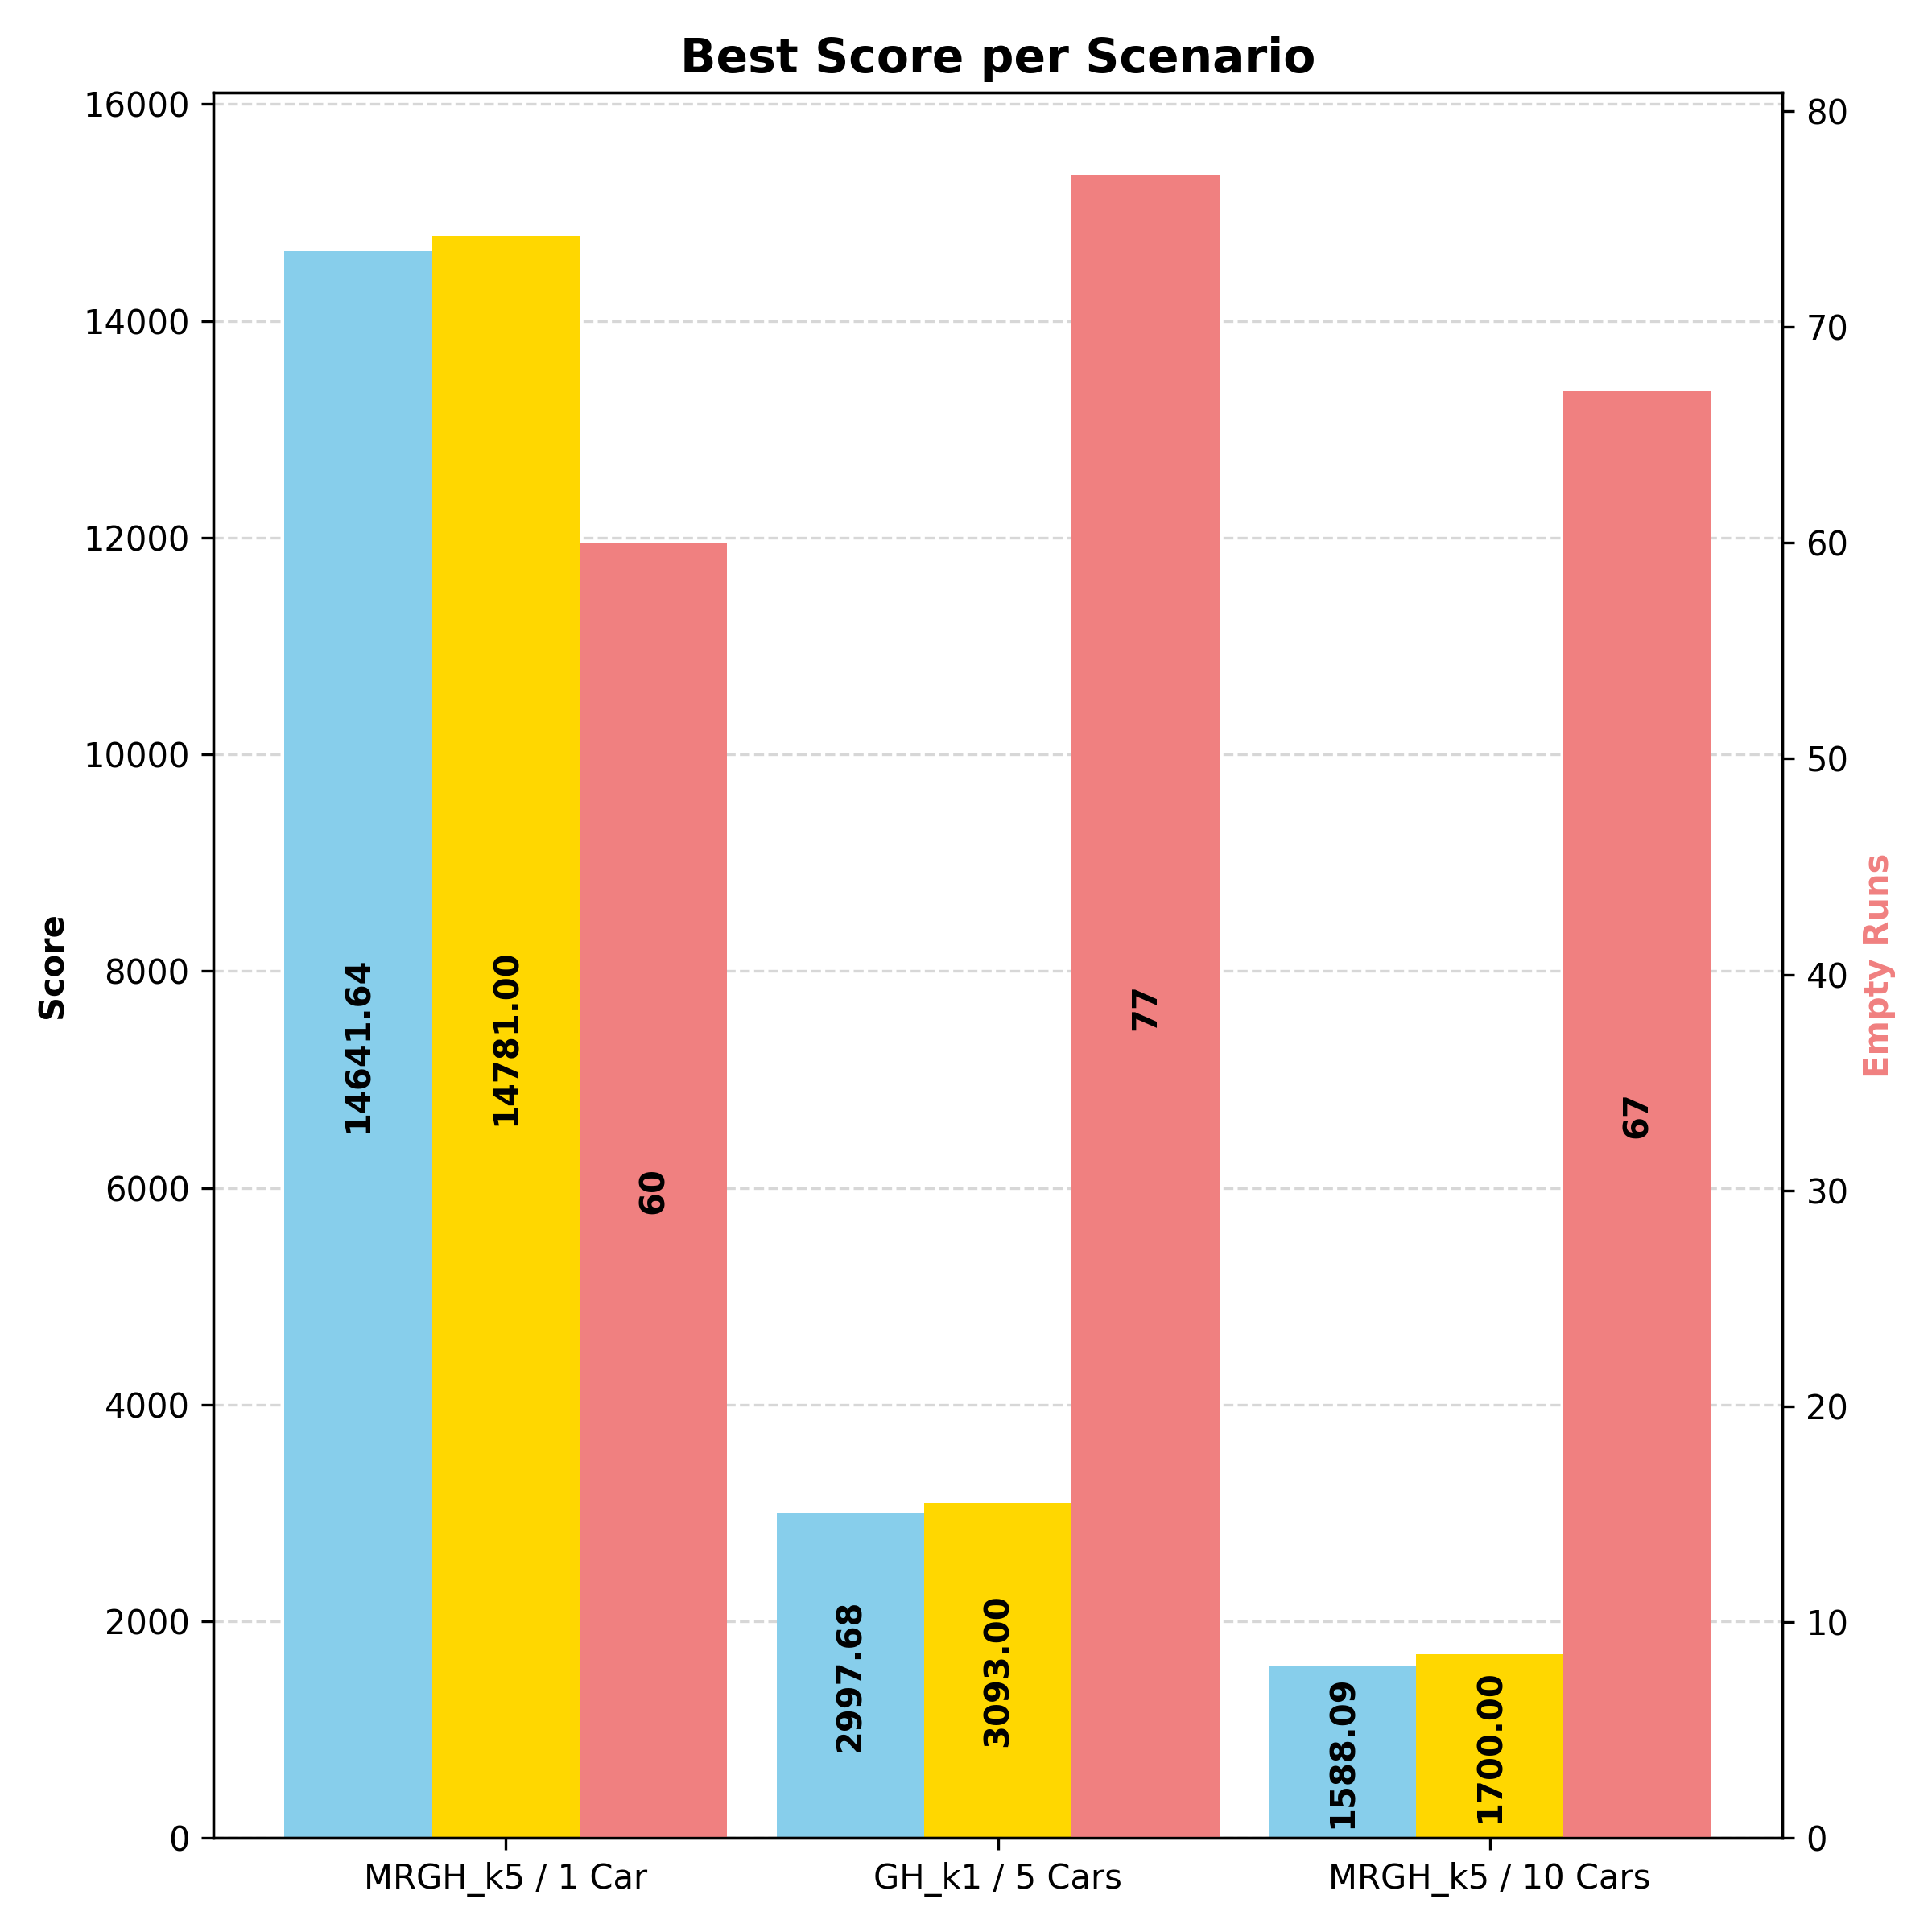
\includegraphics[width=0.9\textwidth]{figures/best_validation_results.png}
  \caption{Beste Validierungsergebnisse pro Szenario im Vergleich zum Kurs-Referenzwert
  sowie die zugehörige Anzahl an Leerfahrten.}
  \label{fig:best_validation_results}
\end{figure}

Die Ergebnisse zeigen, dass die Leistungsfähigkeit der untersuchten Heuristiken stark vom
jeweiligen Szenario abhängt. Während bei mittlerer Fahrzeuganzahl die klassische Greedy-
Heuristik ausreichend ist, profitieren Szenarien mit sehr wenigen oder sehr vielen Fahrzeugen
von der erweiterten Suchstrategie des Multistart Randomized Greedy Ansatzes.

Insgesamt stellt die MRGH einen guten Kompromiss zwischen Lösungsgüte und Rechenaufwand dar,
während die Greedy-Heuristik insbesondere durch ihre Einfachheit und Effizienz überzeugt.

\section*{Hinweis zu verwendeten Hilfsmitteln}
ChatGPT (OpenAI) wurde zur sprachlichen Strukturierung, zur Formulierung einzelner Textpassagen
sowie zur Klärung konzeptioneller Fragestellungen eingesetzt \cite{chatgpt2025}.
GitHub Copilot wurde unterstützend bei der Implementierung und beim Refactoring
von Code verwendet \cite{copilot2025}. Die inhaltliche Verantwortung für Konzeption,
Implementierung und Auswertung liegt vollständig bei den Autoren.


\bibliographystyle{unsrt}
\bibliography{literatur}

\end{document}